\begin{figure}[h]
  \centering
  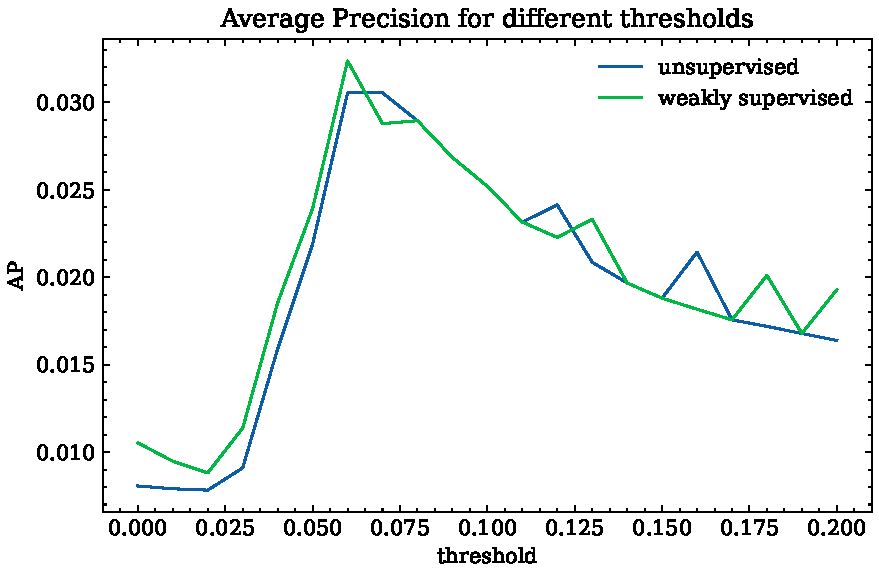
\includegraphics{5Results/figs/bsle/average_precision_score_for_thresholds.pdf}
  \caption{Average Precision scores (higher is better)}
\end{figure}
\begin{figure}[h]
  \centering
  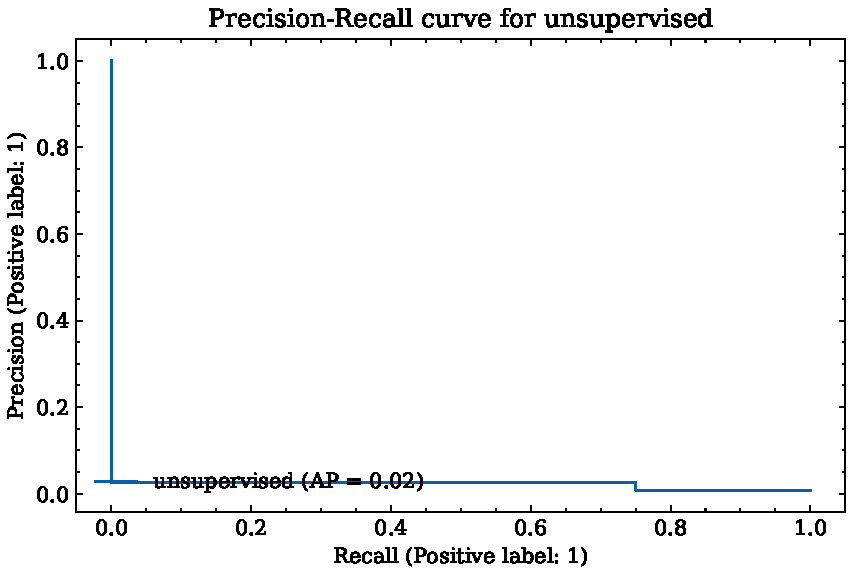
\includegraphics{5Results/figs/bsle/pr_auc_unsupervised.pdf}
  \caption{AP for unsupervised}
\end{figure}
\begin{figure}[h]
  \centering
  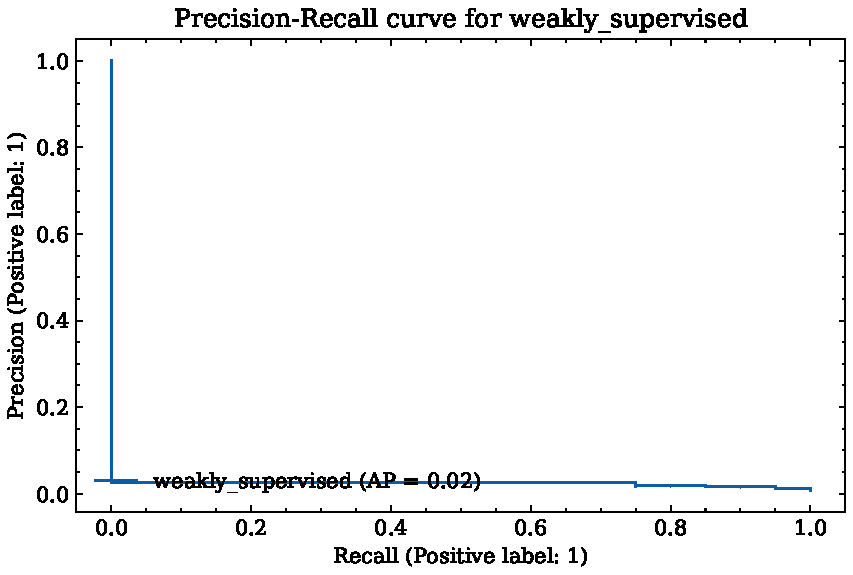
\includegraphics{5Results/figs/bsle/pr_auc_weakly_supervised.pdf}
  \caption{AP for weakly supervised (higher is better)}
\end{figure}
\begin{figure}[h]
  \centering
  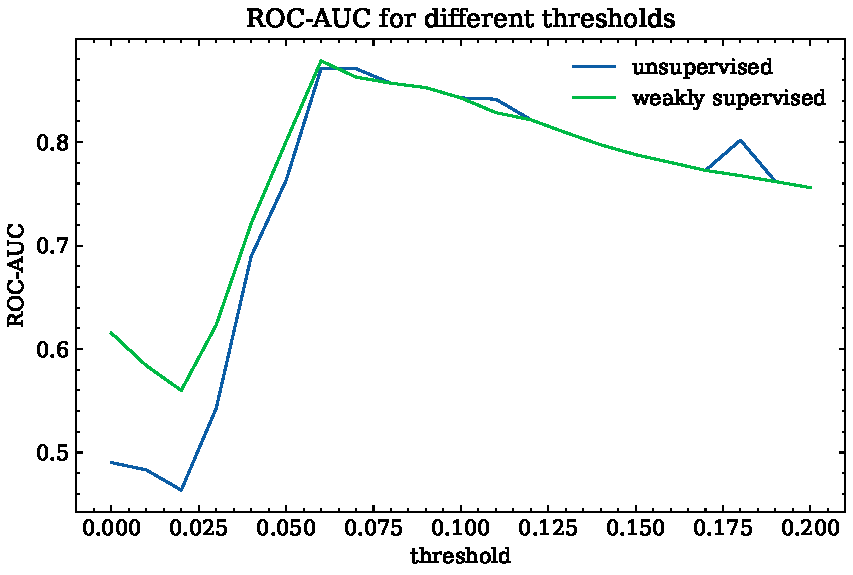
\includegraphics{5Results/figs/bsle/roc_auc_score_for_thresholds.pdf}
  \caption{ROC-AUC scores (higher is better)}
\end{figure}
\begin{figure}[h]
  \centering
  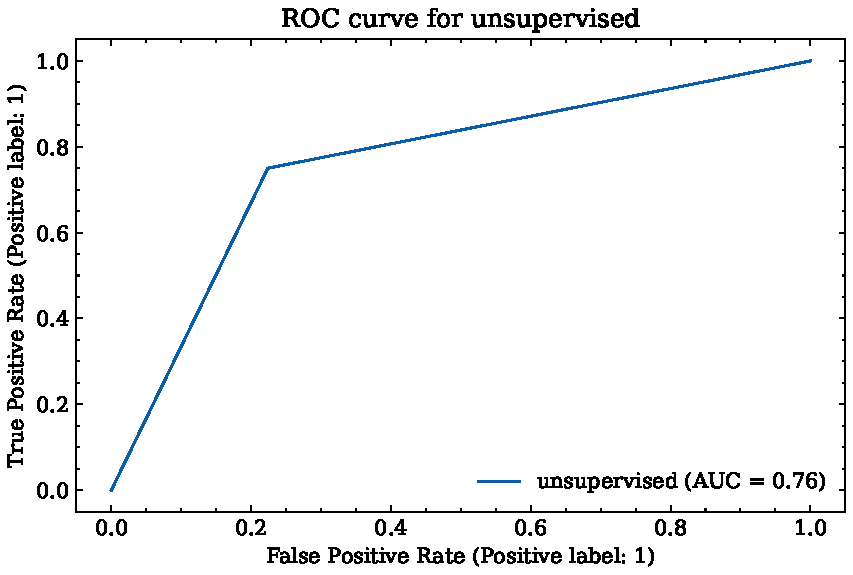
\includegraphics{5Results/figs/bsle/roc_auc_unsupervised.pdf}
  \caption{ROC for unsupervised}
\end{figure}
\begin{figure}[h]
  \centering
  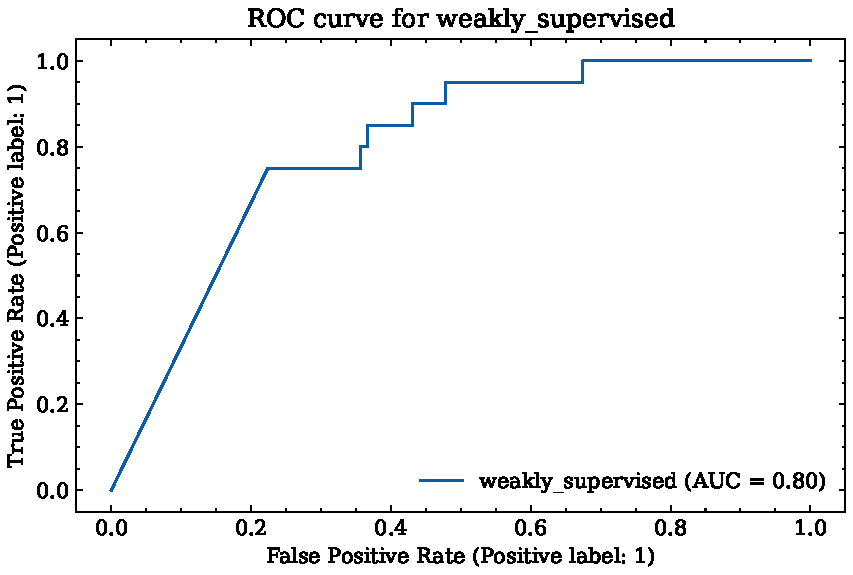
\includegraphics{5Results/figs/bsle/roc_auc_weakly_supervised.pdf}
  \caption{ROC for weakly supervised
  \NS[inline]{add threshold parameter}
  }
\end{figure}
\begin{figure}[h]
\centering
  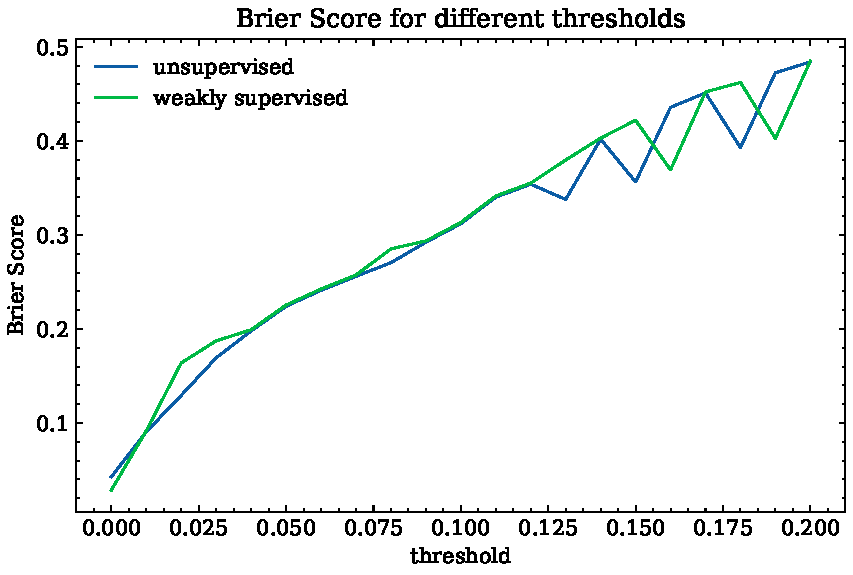
\includegraphics{5Results/figs/bsle/brier_score_for_thresholds.pdf}
  \caption{Brier scores (lower is better)}
\end{figure}
\begin{figure}[h]
\centering
  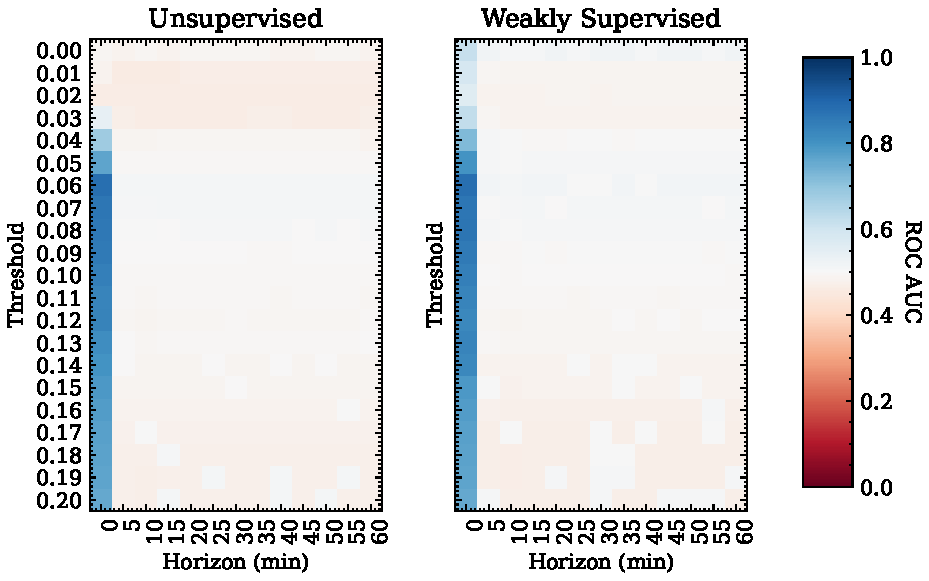
\includegraphics{5Results/figs/bsle/auc_roc_scores_for_thresholds_and_horizons_min.pdf}
  \caption{AUC-ROC Heatmap for minutes time scale}
\end{figure}
\begin{figure}[h]
\centering
  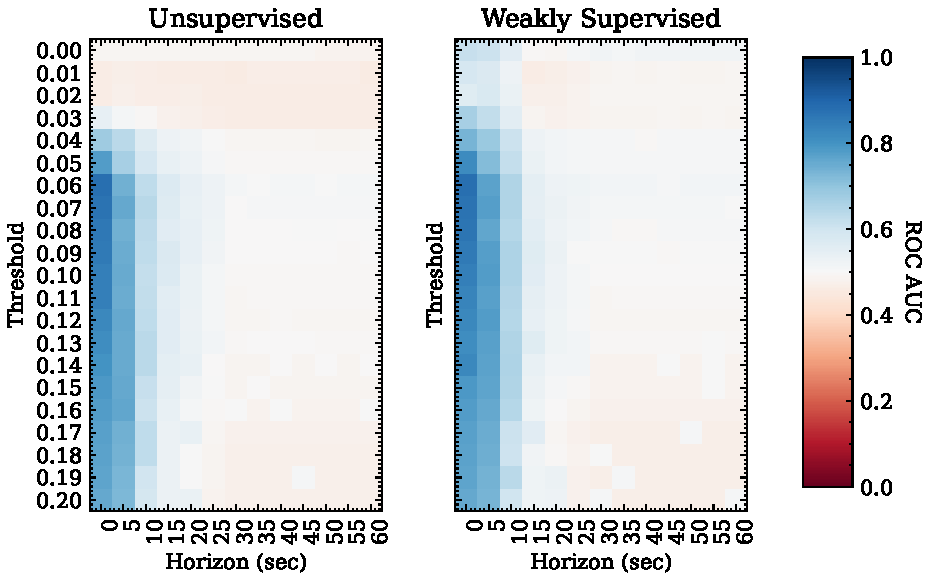
\includegraphics{5Results/figs/bsle/auc_roc_scores_for_thresholds_and_horizons_sec.pdf}
  \caption{AUC-ROC Heatmap for seconds time scale}
\end{figure}
% \Caption{Embedding of EEG}{}
% \label{fig:5results:bsle}

